\documentclass{standalone}

\usepackage{bm}
\usepackage{fontspec}
\usepackage{pslatex}
\usepackage{tikz}

\usetikzlibrary{arrows.meta}
\usetikzlibrary{backgrounds}
\usetikzlibrary{fit}
\usetikzlibrary{matrix}
\usetikzlibrary{positioning}
\usetikzlibrary{shapes.geometric}

\newcommand{\mat}[1]{\bm{#1}}
\newcommand{\Tr}{^{\top}}
\newcommand{\vc}[1]{\bm{#1}}

%\setmainfont{Liberation Sans}
\newlength{\mywidth}
\newlength{\myheight}

\makeatletter
\DeclareRobustCommand{\rvdots}{%
  \vbox{
    \baselineskip4\p@\lineskiplimit\z@
    \kern-\p@
    \hbox{.}\hbox{.}\hbox{.}
  }}
\makeatother

\begin{document}
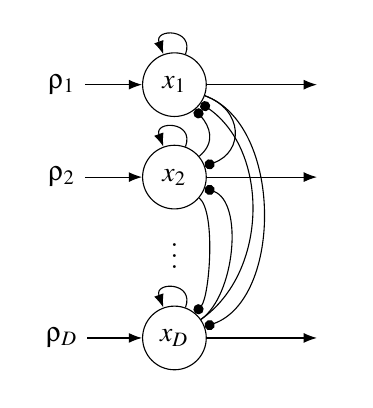
\begin{tikzpicture}[
    every path/.style={-{Latex}},
    inhibit/.style={-{Circle}},
    neuron/.style={circle, minimum size=23, draw=black},
    gate/.style={diamond, draw=black},
    net/.style={rectangle, draw=black},
    ]

    \matrix [column sep=20, row sep=10] {
        \node (rho1) {$\rho_1$}; & \node (x1) [neuron] {$x_1$}; &[20] \node (out1) {}; \\
        \node (rho2) {$\rho_2$}; & \node (x2) [neuron] {$x_2$}; & \node (out2) {}; \\
        & \node {$\rvdots$}; & \\
        \node (rhoD) {$\rho_D$}; & \node (xD) [neuron] {$x_D$}; & \node (outD) {}; \\
    };

    \foreach \i in {1, 2, D} {
        \draw [loop above, min distance=10, in=110, out=70] (x\i) to (x\i);
        \draw (rho\i) to (x\i);
        \draw (x\i) to (out\i);
    }
    \draw (x1) [inhibit, in=20, out=340, distance=15] to (x2);
    \draw (x1) [inhibit, in=20, out=340, distance=30] to (xD);
    \draw (xD) [inhibit, out=35, in=325, distance=30] to (x1);
    \draw (xD) [inhibit, out=35, in=340, distance=15] to (x2);
    \draw (x2) [inhibit, out=40, in=310, distance=8] to (x1);
    \draw (x2) [inhibit, out=320, in=50, distance=8] to (xD);
\end{tikzpicture}
\end{document}
